

\documentclass[runningheads,legalpaper,10pt]{etc/llncs}
\usepackage{amssymb}
\usepackage{graphicx}
\usepackage{hyperref}
\usepackage{booktabs}
\usepackage{url}
\usepackage{float}
\usepackage{chngpage}
\usepackage{listings}
\usepackage{apacite}
\usepackage[backend=biber,style=authoryear,sorting=nty]{biblatex}

\usepackage[utf8]{inputenc}
\usepackage[spanish,activeacute]{babel}

\usepackage{longtable}
\usepackage{makecell}


\let\stdsection\section
\renewcommand\section{\newpage\stdsection}
\addbibresource{citations.bib}

\urldef{\mailsa}\path|federico.scenna@gmail.com|    
\newcommand{\keywords}[1]{\par\addvspace\baselineskip
\noindent\keywordname\enspace\ignorespaces#1}

\authorrunning{Lic. Federico Scenna}% Part of LEFT running header
\titlerunning{Análisis de grafos del mercado de criptomonedas}% Part of RIGHT running header

\mainmatter  % start of an individual contribution

% first the title is needed
\title{Análisis de grafos del mercado de criptomonedas}

\author{Lic. Federico Scenna\\ [1cm] {\small Tutor: Dr. Ricardo Maronna}}


\institute{ Maestría en Exploración de Datos y Descubrimiento del Conocimiento \\
Facultad de Ciencias Exactas y Naturales\\ Universidad de Buenos Aires\\
\mailsa
}
\setcounter{tocdepth}{3}


\begin{document}
\let\oldaddcontentsline\addcontentsline
\def\addcontentsline#1#2#3{}
\maketitle
\def\addcontentsline#1#2#3{\oldaddcontentsline{#1}{#2}{#3}}

\newpage

\paragraph{Resumen} En este trabajo se analizan series diarias de precios de las criptomonedas con mayor capitalización de mercado entre Agosto del año 2020 y Abril de 2021. A partir de correlaciones
de retornos logarítmicos diarios y con una metodología de análisis consistente con la literatura actual, se visualizaron las relaciones entre los distintos activos. Se
identificaron mayoritariamente altas correlaciones entre los movimientos de precios y, a diferencia de otros estudios, ni Bitcoin ni Ethereum fueron los activos de referencia durante el periodo analizado. A su vez, se detectaron dos activos que figuraban desacoplados de la red. 
Adicionalmente, se aplicaron algoritmos de búsqueda de comunidades, siendo el algoritmo de Louvain el de mejores resultados, logrando separar los activos volátiles de los estables.

\paragraph{Palabras clave} Análisis de grafos, mercados financieros, criptomonedas, blockchain

\tableofcontents

\newpage
\section{Introducción}

El mercado de los criptoactivos atraen atención tanto por los medios, los inversores y los organismos regulatorios. Además de la posibilidad de funcionar como dinero digital, existe una variedad de casos de uso potenciales en distintos rubros. En  finanzas, la propuesta más relevante viene desde modelos de finanzas descentralizadas (DeFi). Sin embargo, los casos de uso no se limitan únicamente en finanzas sino que existen potencialidades de innovación en otras ámbitos (desde nuevos casos de uso en productos artísticos hasta mejoras en la trazabilidad de procesos en la industria de retail). En este contexto, los estudios académicos que existen sobre este fenómeno podrían considerarse insuficientes en comparación con la relevancia que tiene esta tecnología en el discurso público. La mayoría de los estudios existentes se centran en estudiar principalmente a Bitcoin, el activo más popular y más antiguo. Sin embargo, segun el sitio CoinMarketCap.com, existen más de 20,280 criptoactivos. De este total, hay 10 criptoactivos con una capitalizacion de mercado mayor a 10 mil millones de dólares.

Existen varios antecedentes de aplicaciones de grafos para analizar dinámicas en el campo de la economía. El trabajo de  \cite{economicsnetworks} compila el estado actual de estas  investigaciones. Adicionalmente, este tipo de análisis tiene la potencialidad de iniciar nuevos tipos de investigaciones, como el impacto de narrativas en los comportamientos de los agentes económicos (\cite{schiller}). Adicionalmente, en la literatura de estudios financieros existen aplicaciones de este tipo de análisis, tanto para estudiar las dinámicas de las finanzas internacionales como la de mercados bursátiles singulares. 

Como ejemplo en finanzas internacionales, en el trabajo de \cite{towards} se aplica análsis de grafos para estudiar la integracion global y la estabilidad de los mercados bursátiles. Los autores concluyen que la integracion global de estos mercados fue en claro retroceso desde el inicio de la Primer Guerra Mundial y fundamentalmente se mantuvo sin cambios durante el periodo entreguerras y hasta fines de las décadas de 1980 y 1990. Esta tendencia fue revertida considerablemente desde entonces y los autores demostraron que si bien en la segunda era de la globalización estos mercados se encuentran altamente integrados pero también con los  mayores niveles de inestabilidad financiera.

A su vez, existen ejemplos de aplicaciones para mercados singulares como \cite{grekmarket}  que han utilizado este tipo de análisis para el mercado bursátil griego. Los autores encontraron algunos grupos de activos altamente correlacionados, lo que permitía inferir un perfil de inversor.

 Las aplicaciones del análisis de grafos para el caso de los criptoactivos, la acotada literatura existente se focaliza en dos aspectos. Por un lado, los criptoactivos se encuentran desarrollados sobre una red distribuida de nodos peer-to-peer que son los que se encargados de validar y registrar las transacciones. En esa dirección, los trabajos de \cite{btc-blockchain} y \cite{btc-btccash} son ejemplos de este foco de estudio. 
 
 Por el otro lado, si bien no abundan los los trabajos de análisis de grafos partiendo de los retornos. Existen dos estudios ejemplificadores. En  \cite{cryptocurrency_rjc} los autores determinaron a Ethereum como el activo de referencia durante el periodo de Julio 2017 y Septiembre 2018. En un estudio más extendido, \cite{cryptonetwork} analizan 120 criptoactivos entre 2013 y 2020. En ese trabajo, determinaron que Bitcoin dominó el mercado hasta mediados del 2016, dominado luego por dos activos (MAID y FCT) desarrollados para implementar aplicaciones de la tecnología blockchain hasta mediados de 2017. Desde entonces Ethereum junto a otros criptoactivos como Cardano, Neo y OMG reemplazaron a Bitcoin como el activo de referencia de la red, principalmente por su capacidad de implementar \emph{smart contracts} (contratos inteligentes) para implementar lógicas de negocio automatizadas. Adicionalmente, encontraron que durante el inicio del Covid-19, QTUM y BNB reemplazaron de manera intermitente a Ethereum como activos de referencia.

En este último sentido, el objetivo de este trabajo es analizar los 45 criptoactivos de mayor volumen de mercado del periodo entre 22 de Agosto 2020 y el 24 de Abril 2021. A partir de ciertas metricas obtenidas a partir de los datos recogidos, se realiza un análisis de grafos con una metodología consistente a la literatura mencionada.

\section{Metodología}

\subsection{Materiales y análisis exploratorio}
 Se descargaron
series de precios del sitio coinmarketcap.com a través de la libreria de R crypto \footnote{Disponible en: $https://www.rdocumentation.org/packages/crypto/versions/1.1.3$}. A través de este paquete de R, se descargaron datos diarios de 45 criptoactivos más activos entre el periodo de análisis y de cada uno de ellos se encontraron disponibles datos de precio máximo, precio mínimo, precio inicial, volumen y precio de cierre.


A partir de este dataset, se generó una lista para identificar a los activos tanto volátiles como estables (estos últimos fueron diseñados para mantener un valor similar al dólar estadounidense). Esta lista resultó de utilidad para poder generar visualizaciones y analizar los grafos.
Tanto los datos como el código de este trabajo se encuentran disponibles un repositorio de Github\footnote{$https://github.com/FedeScenna/Crypto_NetworkAnalysis$}.

Las figuras \ref{fig:volatile} y \ref{fig:stablecoins} muestran el precio de cierre de los activos volátiles y estables respectivamente.  En el caso del comportamiento de los activos volátiles es llamativo el comportamiento del activo YFI (de Yearn Finance, un proyecto de finanzas descentralizadas). Durante el periodo que se toma de análisis para este trabajo este activo alcanzó excepcionalmente valores similares en tendencia al Bitcoin.

\subsection{Transformacion de datos}

Previamente a la construcción del grafo, era necesario establecer alguna métrica para desestacionalizar la serie de precios de los activos para evitar correlaciones espurias. Uno de los métodos más frecuentes que propone la literatura \cite{cryptonetwork} es la tasa de retorno logarítmica:

\[
\log(p_t) - \log(p_{t-1})
\]


Se decidió, a modo de mantener la claridad en el análisis y por las cualidades
propias del este tipo de mercado, computar retornos diarios de cada uno de los
activos. La distribución del mismo para cada uno de los activos se puede visualizar en la figura \ref{fig:box_returns}. Lo más resaltable de este gráfico es la dispersión del retorno de algunos activos (como HEX o HEDG) que no forman parte de las carteras mas tradicionales de inversiones.

Además del retorno promedio o esperado de cada uno de los activos, la volatilidad es otro de los factores relevantes para las decisiones  y la conformación de una cartera de inversión (\cite{randomwalkdownstreet}). En la figura \ref{fig:risk_matrix} podemos observar la matriz de riesgo-retorno \footnote{Para mayor detalle, en el repositorio de Github de este proyecto hay un gráfico interactivo para consultar}. El punto de corte para clasificar a cada uno de los activos se calcula respecto a las posiciones de cada activo respecto de las medianas de retorno y volatilidad de todo el panel de activos. De esta manera, se pueden segmentar los activos en cuatro grupos:

\begin{itemize}
    \item Alto retorno, alto riesgo
    \item Bajo retorno, alto riesgo
    \item Alto retorno, bajo riesgo
    \item Bajo retorno, bajo riesgo
\end{itemize}

A partir de estos resultados, hay algunos resultados relevantes. En primer lugar, CTC y HEX son dos activos de alto retorno y alta volatilidad que se encuentran ampliamente alejados de su propio cuadrante. Luego, HEDG y CRO (de bajo retorno y alto riesgo) son los activos más llamativos de su cuadrante). FTT, por su lado, es el activo más importante en términos de alto retorno y bajo riesgo. Cada uno de estos resultados está en sintonía con sus características cualitativas. Fundamentalmente la propuesta de valor del mismo. Mientras CTC se trata de un proyecto de microfinanzas, HEX es un proyecto de finanzas descentralizadas (en la jerga, DeFi) que ha sufrido cuestionamientos de la viabilidad del proyecto a largo plazo. Por el otro lado, HEDG es un proyecto de apuestas via blockchains y FTT es un proyecto del exchange FTX que sigue el valor de activos futuros y derivados \footnote{Al momento de escribir este trabajo, el exchange FTX se ha declarado en bancarrota y el proyecto FTT ha sido descontinuado}. 

Respecto al cuadrante restante, de bajo retorno y bajo riesgo, el mismo se encuentra dominado por las monedas estables que siguen el valor del dólar estadounidense.

La tabla \ref{tab:desc_stats} muestra un resumen estadistico de los retornos para los distintos activos. A partir de esta información, es notorio que los rendimientos promedios son bajos o en algunos casos nulos. Sin embargo, debido a la dispersión de rendimientos, resultan llamativos dos casos: CTC que alcanzó un alza diaria de 384\% y HEX con una baja de -100.4\%.

A partir de esta métrica de retorno, se calculó la matriz a partir de la correlación de Pearson (ver figura \ref{fig:corr_matrix}). Adicionalmente, se puede ver la distribución de las correlaciones de esta matriz en la figura \ref{fig:hist_corr}. A partir de estos gráficos, se concluye que las distribución de las correlaciones tienen una forma bimodal.

\section{Resultados}


\subsection{Clusters de series de tiempo}

Como primer enfoque, se optó por hacer una clusterización. Dado que los datos disponibles son series de tiempo, existen métodos específicos para realizar aprendizaje no supervisado sobre los mismos. Las series de tiempo por definición son datos indexados en un orden temporal y, por lo tanto, calcular su similitud usando una métrica de distancia euclediana no es lo más adecuado porque calcula similitudes en el espacio para el mismo punto temporal para todas las series. Sin embargo, las mismas pueden no coincidir en el espacio temporal, su velocidad o pueden tener una longitud distinta. Como solución a este tipo de problemas, existe otra métrica con la cual calcular distancia: Dynamic Time Wrapping (DTW). 

A partir de la misma, se utiliza un modelo de K-Means (DTW+KMeans) seleccionando un valor de clusters óptimo según la regla del codo, bajo la cuál se estima la cantida de clusters minimizando la métrica de perdida (en este caso, WCSSS o Within Cluster Sum of Squares) a partir del punto en el cual deja de disminuir significativamente (ver figura \ref{fig:knee_cluster}). 
Como resultado, se obtuvieron cinco clústers distintos que se pueden observar en la figura \ref{fig:DTW_clusters}. 

Para cada uno de los clusters se crearon matrices de riesgo-retorno (ver figuras \ref{fig:cluster_1}, \ref{fig:cluster_2}, \ref{fig:cluster_3}, \ref{fig:cluster_4} y \ref{fig:cluster_5}). 
El primero de los resultados, a diferencia de los hallazgos hasta este momento del trabajo, es la separación en diferentes clusters de las monedas estables. BUSD, USDC y USDT se encuentran en un cluster (figura \ref{fig:cluster_5}), mientras que DAI y TUSD se encuentran en otro (figura \ref{fig:cluster_2}).

\subsection{Visualizaciones} 


En la literatura, la metodología usualmente propuesta es la creación de un grafo a partir de una matriz de correlación con un punto de corte determinado.

En base a la distribución de la correlación, la centralidad y la centralidad de intermediación o betweenness centrality ( ver figuras \ref{fig:hist_corr}, \ref{fig:degree_centrality} y \ref{fig:btw_centrality}) promedio de la red, se tomo como valor de corte las aristas entre activos con una correlación mayor al 20\%. 

Si bien existe un valor de correlación entre cada uno de los activos, tiene sentido tomar las correlaciones más significativas para que el grafo tenga interpretabilidad analítica. En la figura \ref{fig:hist_corr} a partir de una correlación de 0.2, se concentran una gran cantidad de interacciones entre todos los activos. 

El segundo motivo por el cual fue elegido este punto de corte es porque el valor de centralidad de intermediación tiene un máximo local en ese punto de correlación. En otras palabras, los activos en la red poseen caminos más cortos respecto al resto de los activos representados. 
Adicionalmente, en el punto de corte elegido, la red conserva una centralidad promedio lo suficientemente alta como para tener interpretabilidad entre las interacciones.

A partir de este punto de corte y de acuerdo a la metodología de otros proyectos de investigación, se construyó un Minimum Spanning Tree (MST) que puede visualizarse a continuación en la figura \ref{fig:mst}:

A partir de esta estructura, se puede visualizar las distancias relativas de los nodos en función de la correlación que tienen entre si. De tal manera, cuan más cerca se encuentren dos nodos mayor es la correlación que existe entre ellos. 

\subsection{Búsqueda de comunidades}

Una herramienta recurrente en el análisis de grafos es la búsqueda de comunidades. Según \cite{networkscience}, se define como comunidad a un grupo de nodos que poseen una probabilidad más alta de conectarse entre sí respecto a otros nodos. Para la búsqueda de comunidades se emplearon dos algoritmos: Louvain y Girvan-Neuman. 

Del resultado de ambos se tomo el algoritmo que arrojaba modularidad más alta. El ganador fue el algoritmo Louvain (figura \ref{fig:community_louvain}) cuya modularidad de 0.68 arrojó mejores resultados que Girvan-Neuman (ver figura \ref{fig:community_gn}). En la imagen siguiente se puede visualizar el resultado de las comunidades encontradas por este algoritmo. El mismo pudo separar adecuadamente los activos estables de los volátiles.

\section{Conclusiones}

En el caso puntual de este trabajo, hay algunas cualidades que deben resaltarse. En primer lugar, se diferencia claramente entre las monedas estables (resaltadas en verde) y las monedas volátiles (en rojo). 

En segundo lugar, observamos que hay dos activos que se encuentran visiblemente desacoplados del resto de los activos del grafo: CTC (Creditcoin) y HEX (Hex.com). El primero es un token de una blockchain destinada a facilitar capital de crédito y trazabilidad de transacciones a fintechs y a proyectos de microfinanzas. El segundo es un proyecto de finanzas descentralizadas destinado a ofrecer alto interés por depósitos a plazo fijo. Sin embargo, han surgido algunas opiniones cuestionando que pueda afianzarse como un proyecto a largo plazo.

En tercer lugar, se puede observar 4 subgrafos de activos que se encuentran conectados entre sí. Lo que es particularmente interesante son los tres subgrafos de monedas volátiles ya que ni ETH ni BTC son los activos de referencia de esos subgrafos. De esta manera, se constituye una discrepancia respecto a la literatura consultada para este trabajo.
Adicionalmente, hay activos que sirven de asosiación para cada uno de los subgrafos. LINK cumple la función de activo intermedio entre las monedas estables y el resto de los activos volátiles.

Por último, este trabajo se apoya sobre una literatura disponible escasa y estas conclusiones pueden servir como punto de partida para extender este análisis a otros periodos, analizar una cartera distinta de criptoactivos y expandir el repertorio de técnicas utilizadas. 

\printbibliography %[citations]

\section{Apéndice de gráficos y tablas}
\begin{table}[htbp]
  \centering
  \caption{Estadísticas resumen de los criptoactivos}
  \begin{tabular}{lrrrrrr}
    \toprule
    \multicolumn{1}{c}{\textbf{Activo}} & \multicolumn{1}{c}{\textbf{Máximo}} & \multicolumn{1}{c}{\textbf{Promedio}} & \multicolumn{1}{c}{\textbf{Mínimo}} & \multicolumn{1}{c}{\textbf{Asimetría}} & \multicolumn{1}{c}{\textbf{Desvío Est.}} & \multicolumn{1}{c}{\textbf{Curtosis}} \\
    \midrule
    ADA   & 0.287 & 0.009 & -0.199 & 0.599 & 0.067 & 2.150 \\
    ALGO  & 0.328 & 0.003 & -0.282 & 0.221 & 0.071 & 2.228 \\
    ATOM  & 0.288 & 0.005 & -0.289 & 0.350 & 0.073 & 2.229 \\
    BCH   & 0.275 & 0.004 & -0.229 & 0.008 & 0.061 & 3.893 \\
    BNB   & 0.533 & 0.013 & -0.270 & 1.689 & 0.074 & 11.369 \\
    BSV   & 0.459 & 0.001 & -0.278 & 1.085 & 0.064 & 12.194 \\
    BTC   & 0.178 & 0.006 & -0.141 & 0.164 & 0.038 & 2.640 \\
    BUSD  & 0.003 & -0.000 & -0.003 & -0.132 & 0.001 & 3.668 \\
    CRO   & 0.484 & -0.000 & -0.368 & 0.913 & 0.065 & 15.975 \\
    CTC   & 3.842 & 0.025 & -0.136 & 14.254 & 0.252 & 215.733 \\
    DAI   & 0.016 & -0.000 & -0.016 & 0.443 & 0.002 & 15.898 \\
    DASH  & 0.454 & 0.004 & -0.221 & 1.316 & 0.069 & 8.807 \\
    DOT   & 0.460 & 0.010 & -0.215 & 1.606 & 0.076 & 6.527 \\
    EOS   & 0.156 & 0.002 & -0.227 & -0.157 & 0.059 & 1.961 \\
    ETC   & 0.365 & 0.006 & -0.201 & 1.063 & 0.071 & 5.205 \\
    ETH   & 0.233 & 0.007 & -0.215 & -0.247 & 0.051 & 2.546 \\
    FTT   & 0.277 & 0.011 & -0.172 & 0.586 & 0.053 & 3.758 \\
    HEDG  & 1.288 & -0.002 & -0.319 & 5.814 & 0.123 & 54.499 \\
    HEX   & 1.038 & 0.007 & -1.004 & -0.084 & 0.228 & 5.819 \\
    HT    & 0.487 & 0.005 & -0.220 & 1.839 & 0.062 & 16.346 \\
    LEO   & 0.124 & 0.002 & -0.109 & 0.554 & 0.021 & 13.573 \\
    LINK  & 0.256 & 0.004 & -0.204 & 0.132 & 0.068 & 0.858 \\
    LTC   & 0.169 & 0.006 & -0.200 & -0.127 & 0.056 & 1.329 \\
    MIOTA & 0.281 & 0.006 & -0.202 & 0.361 & 0.065 & 2.380 \\
    MKR   & 0.432 & 0.008 & -0.208 & 1.888 & 0.068 & 9.799 \\
    NEO   & 0.244 & 0.007 & -0.207 & 0.148 & 0.064 & 1.600 \\
    OKB   & 0.493 & 0.004 & -0.231 & 2.629 & 0.070 & 17.680 \\
    OMG   & 0.235 & 0.000 & -0.255 & 0.123 & 0.075 & 1.024 \\
    ONT   & 0.167 & 0.002 & -0.278 & -0.623 & 0.067 & 1.789 \\
    SNX   & 0.186 & 0.004 & -0.243 & 0.057 & 0.076 & 0.179 \\
    THETA & 0.259 & 0.013 & -0.208 & 0.426 & 0.072 & 0.980 \\
    TRX   & 0.344 & 0.006 & -0.188 & 0.837 & 0.064 & 4.037 \\
    TUSD  & 0.003 & 0.000 & -0.005 & -0.232 & 0.001 & 1.243 \\
    UMA   & 0.468 & 0.005 & -0.422 & 1.228 & 0.100 & 6.449 \\
    USDC  & 0.003 & 0.000 & -0.003 & 0.056 & 0.001 & 2.061 \\
    USDT  & 0.003 & 0.000 & -0.003 & -0.044 & 0.001 & 1.058 \\
    VET   & 0.290 & 0.010 & -0.255 & 0.371 & 0.079 & 1.302 \\
    WBTC  & 0.187 & 0.006 & -0.141 & 0.314 & 0.041 & 3.270 \\
    XEM   & 0.250 & 0.005 & -0.459 & -0.515 & 0.079 & 5.838 \\
    XLM   & 0.585 & 0.006 & -0.246 & 2.332 & 0.079 & 14.107 \\
    XMR   & 0.224 & 0.005 & -0.164 & 0.192 & 0.050 & 3.071 \\
    XRP   & 0.451 & 0.006 & -0.538 & 0.371 & 0.089 & 10.223 \\
    XTZ   & 0.197 & 0.001 & -0.199 & -0.175 & 0.059 & 1.699 \\
    YFI   & 0.377 & 0.005 & -0.211 & 0.780 & 0.090 & 1.835 \\
    ZEC   & 0.209 & 0.004 & -0.289 & -0.305 & 0.065 & 2.019 \\
    \bottomrule
    \end{tabular}%
  \label{tab:addlabel}%
\end{table}%

\begin{figure}[htp]
    \centering
    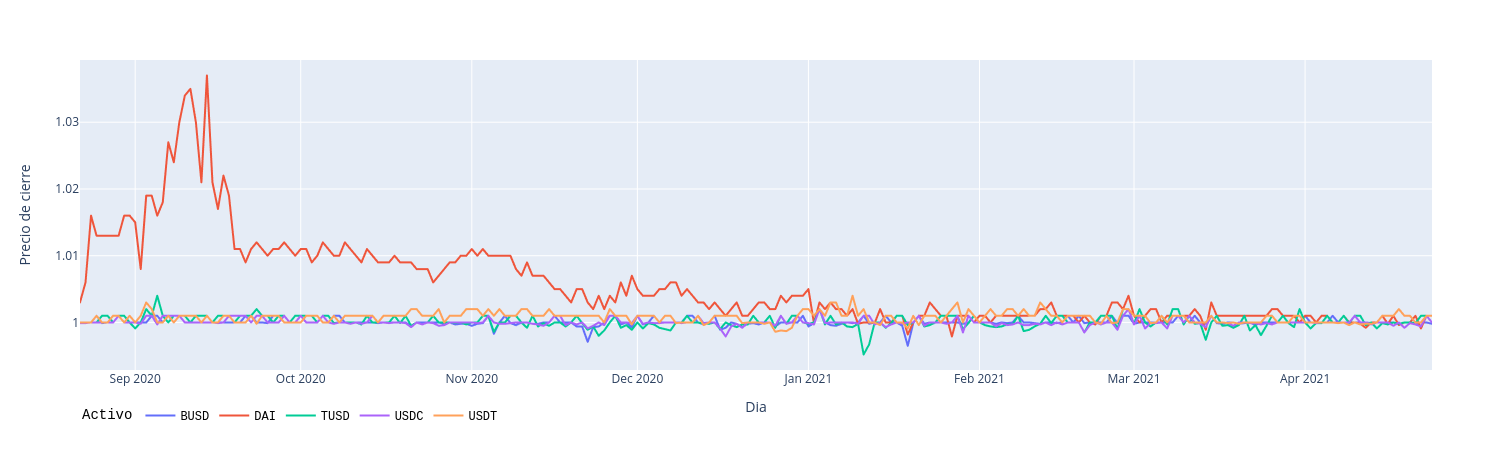
\includegraphics[scale=0.3]{images/stablecoins_lineplot.png}
    \caption{Precios de monedas estables}
    \label{fig:stablecoins}
\end{figure}

\begin{figure}[htp]
    \raggedleft
    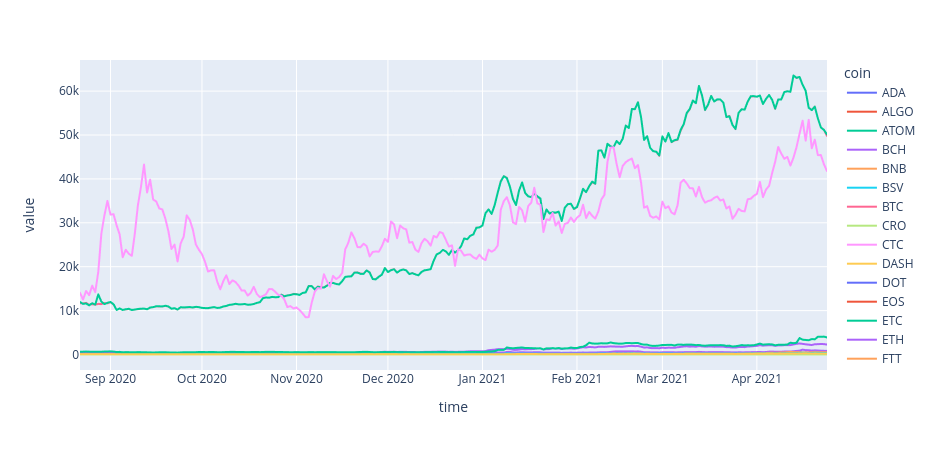
\includegraphics[scale=0.3]{images/volatilecoins_lineplot.png}
    \caption{Precios de monedas volátiles}
    \label{fig:volatile}
\end{figure}

\begin{figure}[htp]
    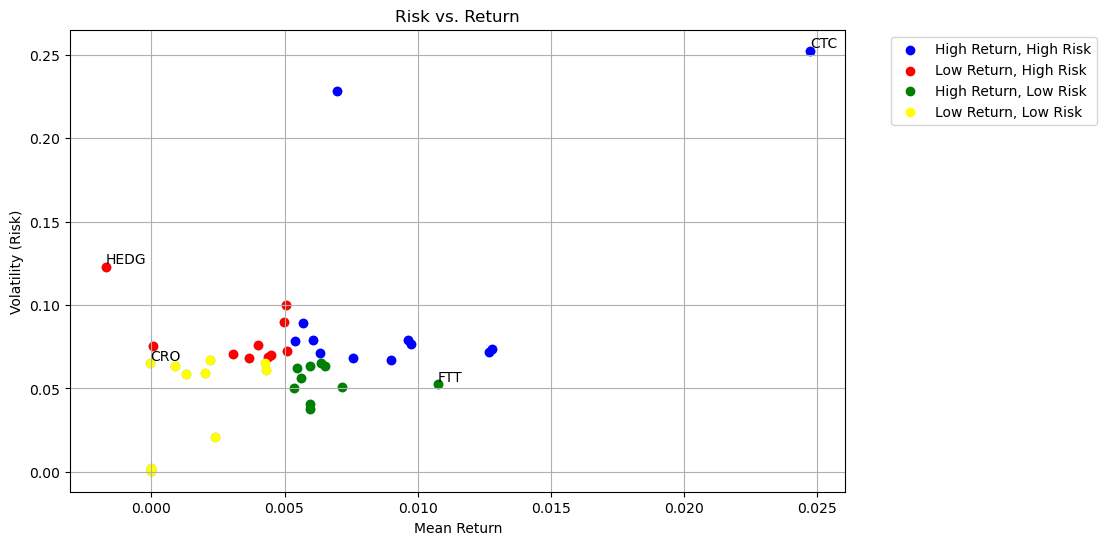
\includegraphics[scale=0.6]{images/risk_matrix.png}
    \caption{Matriz de riesgo-retorno de los activos}
    \label{fig:risk_matrix}
\end{figure}

\begin{figure}[htp]
    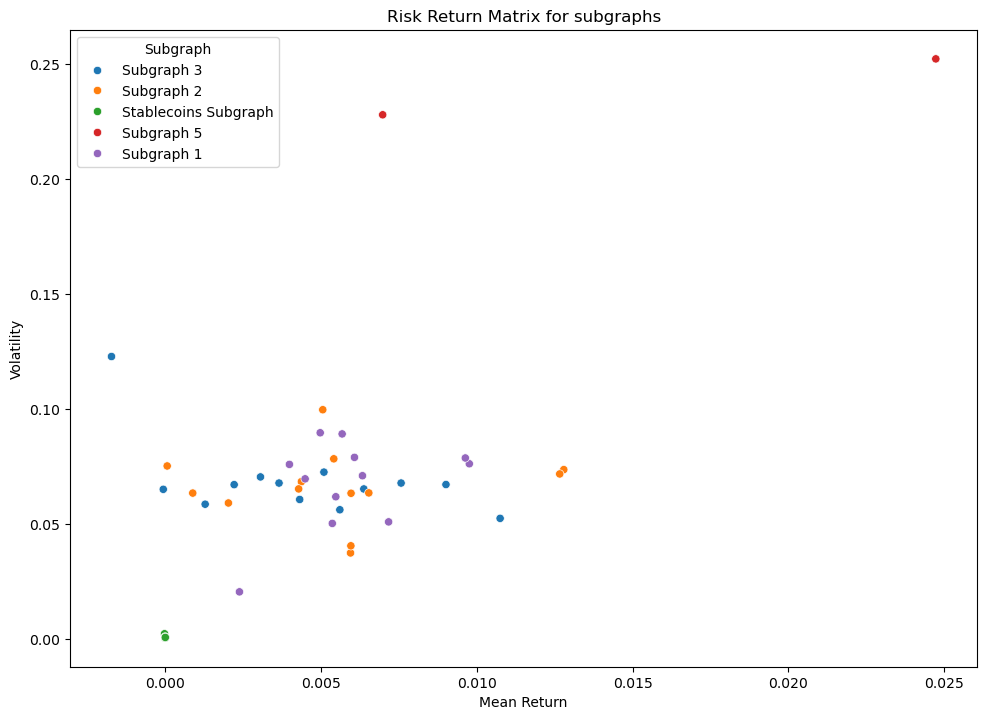
\includegraphics[scale=0.6]{images/risk_matrix_subgraphs.png}
    \caption{Matriz de riesgo-retorno de los activos en subgrafo}
    \label{fig:risk_matrix_subgraph}
\end{figure}

\begin{figure}[htp]
    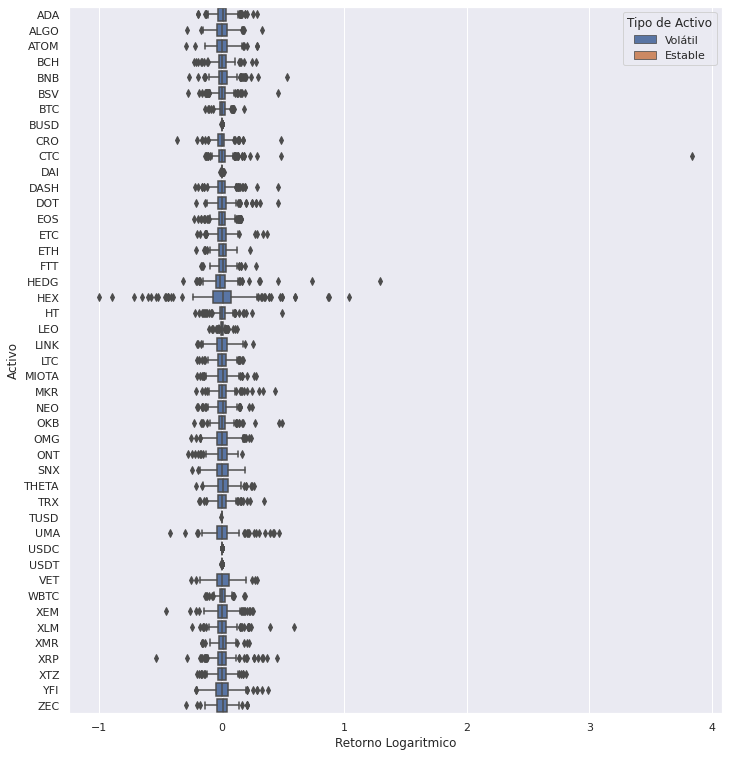
\includegraphics[scale=0.6]{images/box_returns.png}
    \caption{Boxplot de los retornos de los criptoactivos}
    \label{fig:box_returns}
\end{figure}

\begin{figure}[htp]
    \centering
    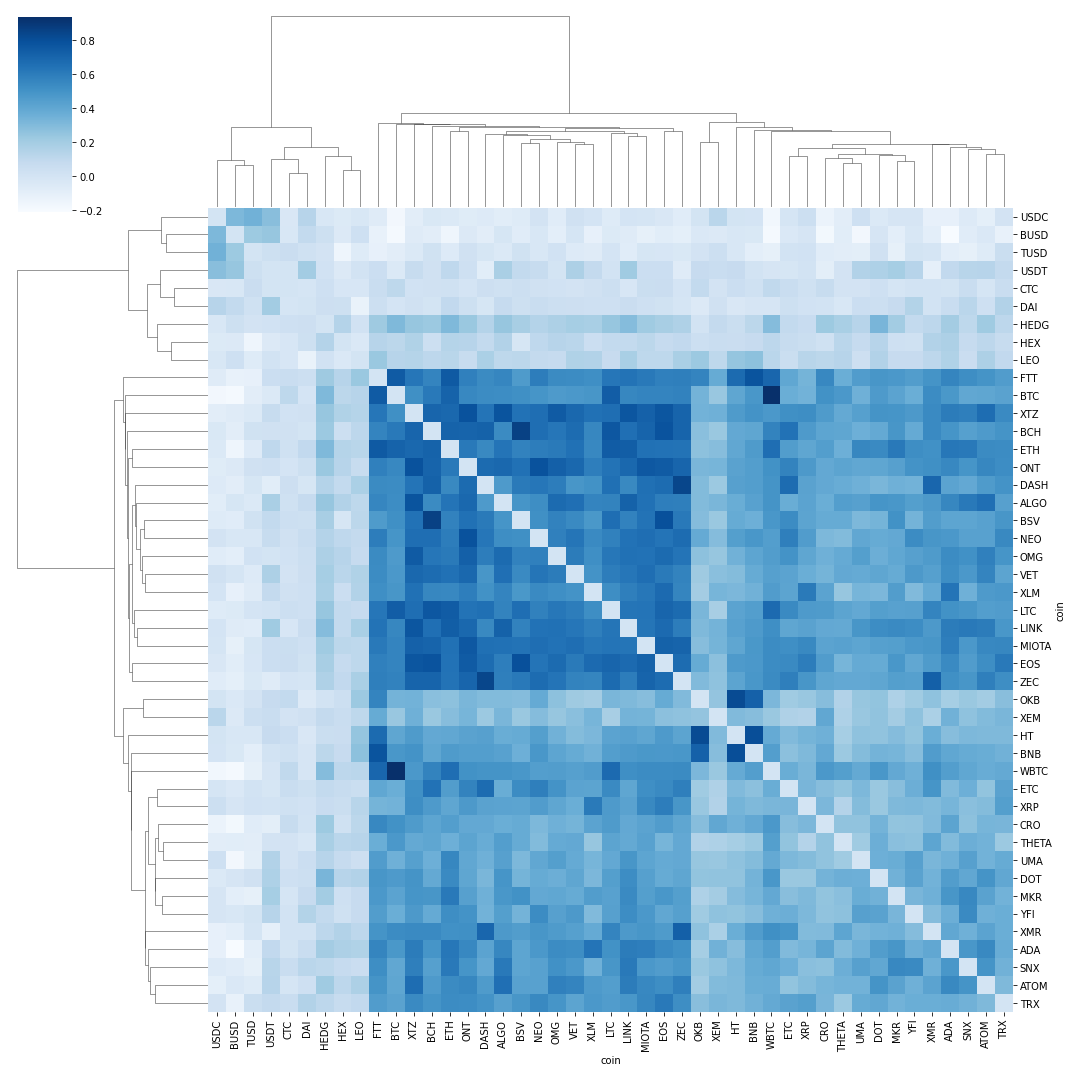
\includegraphics[scale=0.5]{images/corr_matrix.png}
    \caption{Matriz de correlación de los activos}
    \label{fig:corr_matrix}
\end{figure}

\begin{figure}[htp]
    \centering
    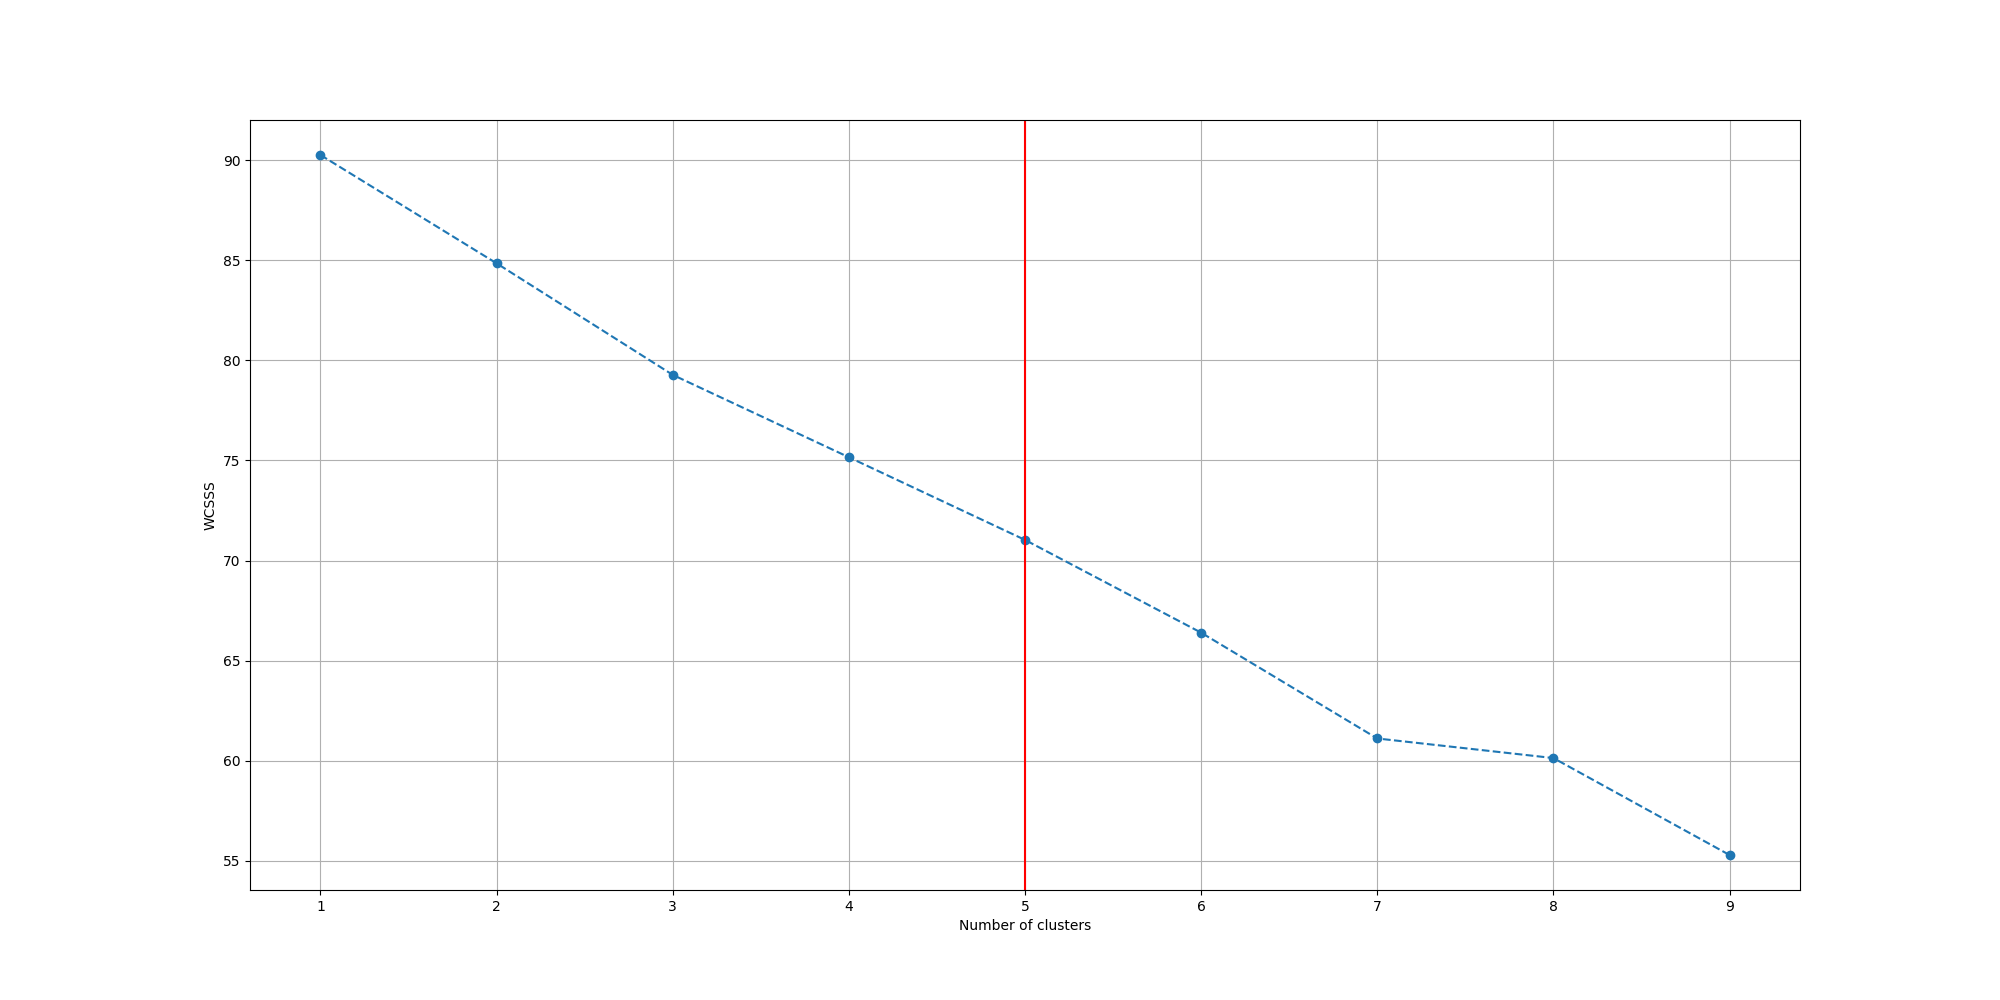
\includegraphics[scale=0.35]{images/knee_cluster.png}
    \caption{Punto de corte para clustering}
    \label{fig:knee_cluster}
\end{figure}

\begin{figure}[htp]
    \centering
    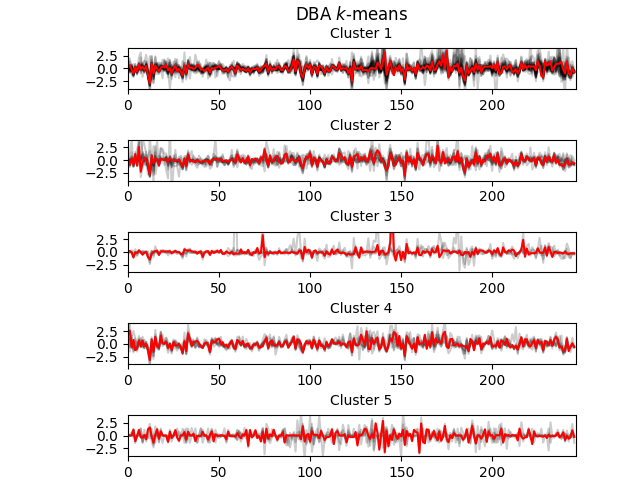
\includegraphics[scale=0.9]{images/DTW_clusters.png}
    \caption{Baricentros de clusters DTW-KMeans}
    \label{fig:DTW_clusters}
\end{figure}

\begin{figure}[htp]
    \centering
    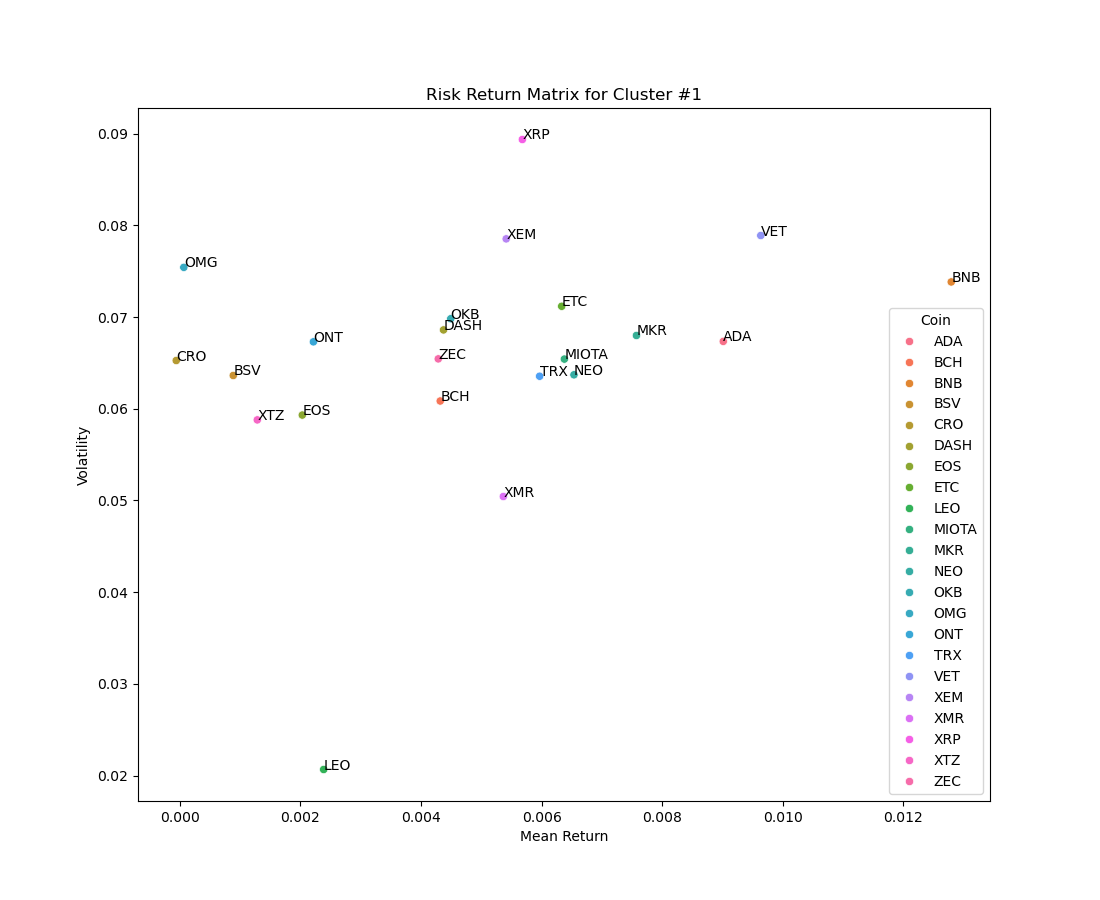
\includegraphics[scale=0.5]{images/cluster_1.png}
    \caption{Matriz riesgo retorno Cluster 1}
    \label{fig:cluster_1}
\end{figure}

\begin{figure}[htp]
    \centering
    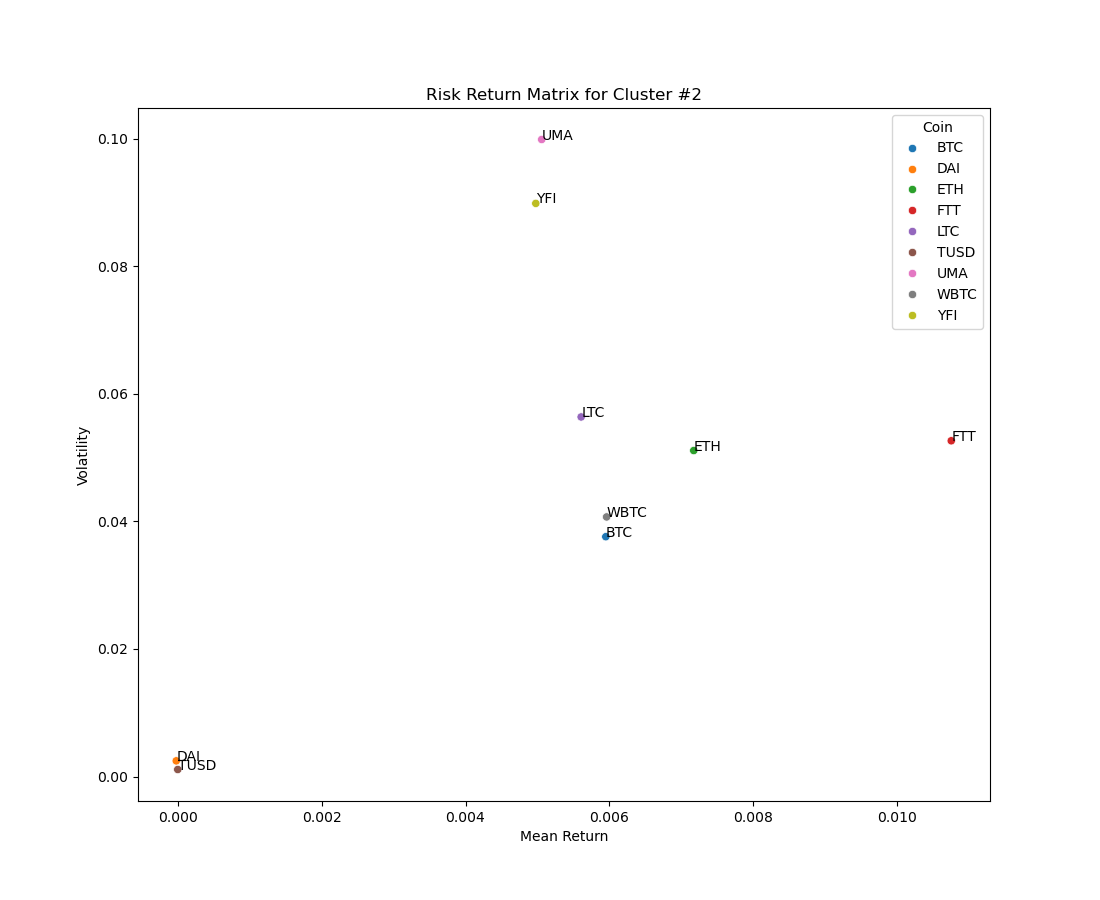
\includegraphics[scale=0.5]{images/cluster_2.png}
    \caption{Matriz riesgo retorno Cluster 2}
    \label{fig:cluster_2}
\end{figure}

\begin{figure}[htp]
    \centering
    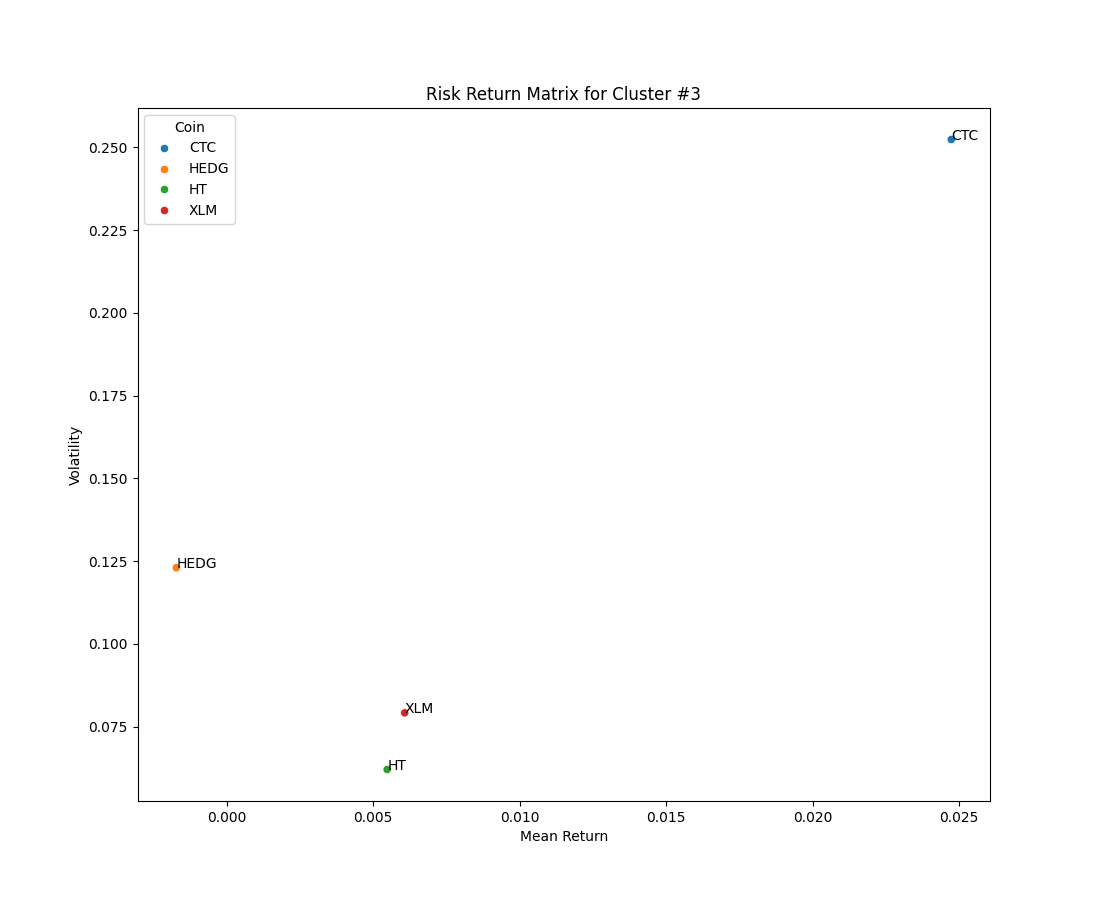
\includegraphics[scale=0.5]{images/cluster_3.png}
    \caption{Matriz riesgo retorno Cluster 3}
    \label{fig:cluster_3}
\end{figure}

\begin{figure}[htp]
    \centering
    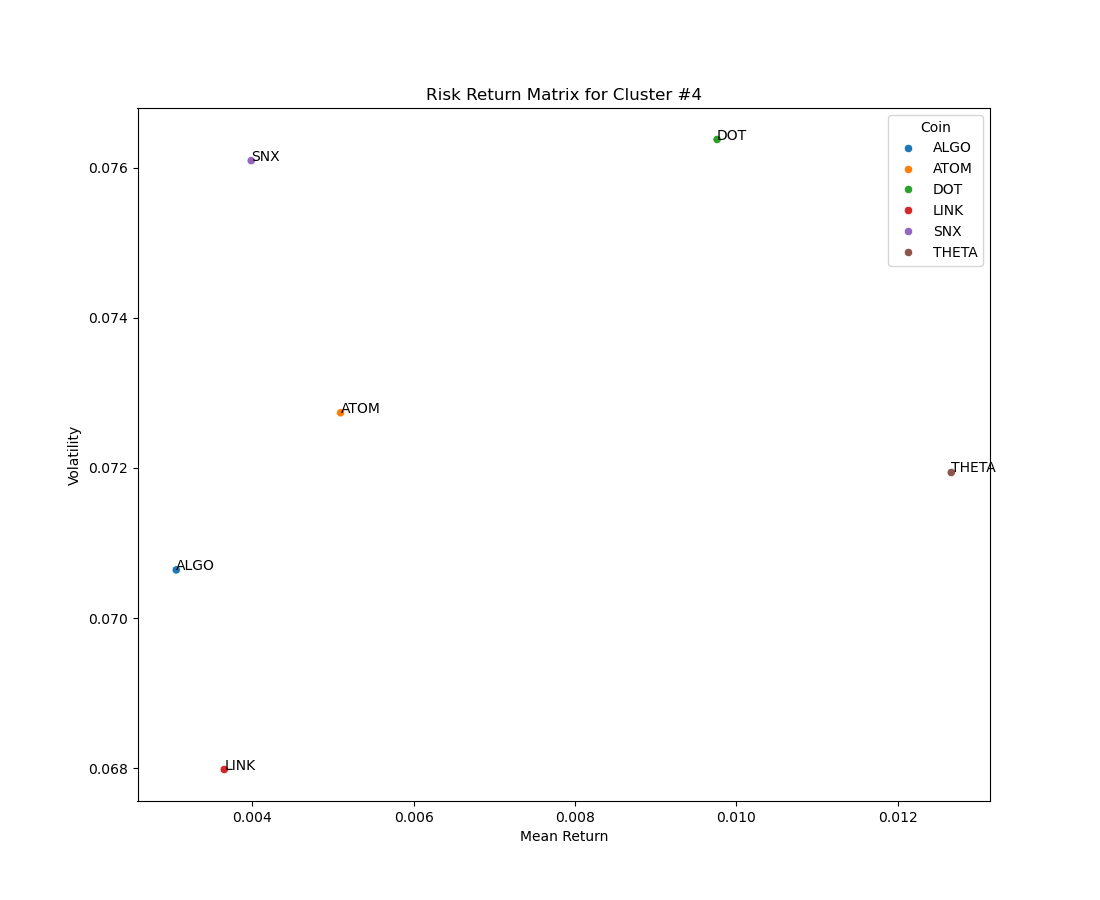
\includegraphics[scale=0.5]{images/cluster_4.png}
    \caption{Matriz riesgo retorno Cluster 4}
    \label{fig:cluster_4}
\end{figure}

\begin{figure}[htp]
    \centering
    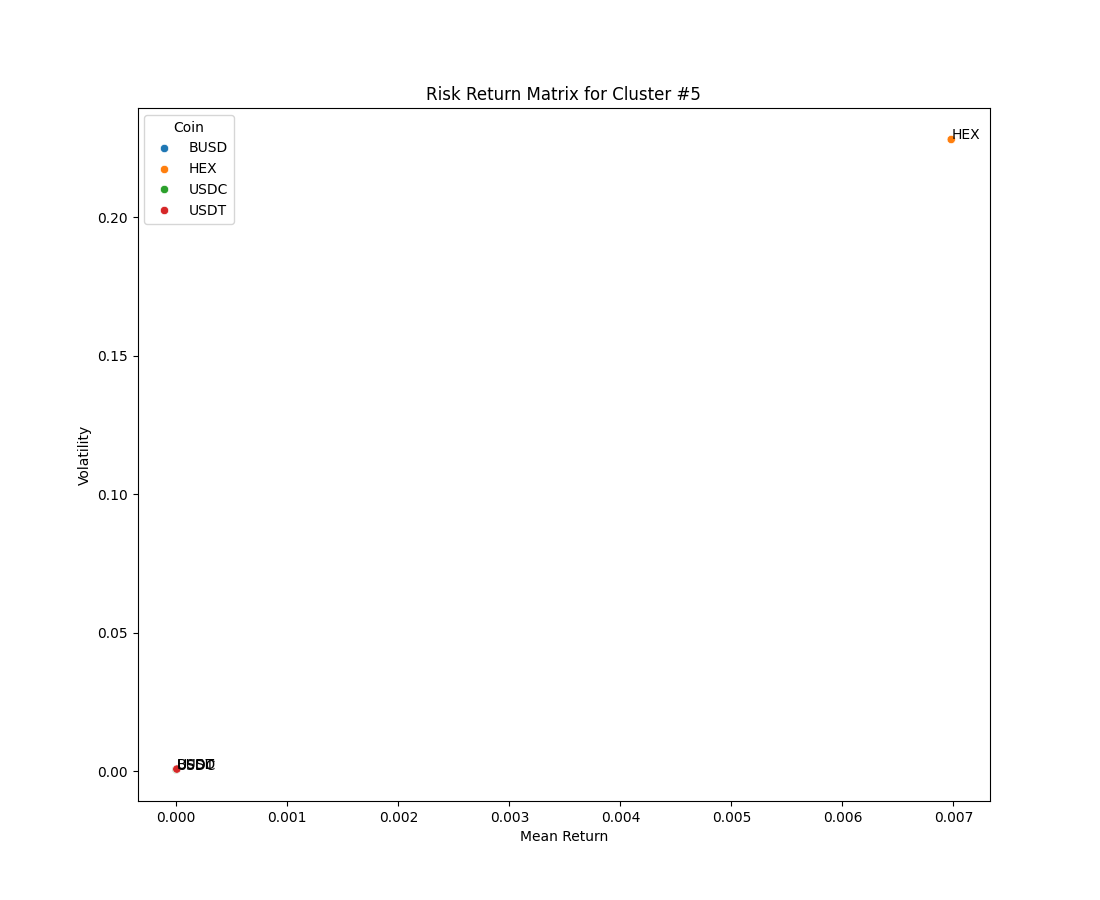
\includegraphics[scale=0.5]{images/cluster_5.png}
    \caption{Matriz riesgo retorno Cluster 5}
    \label{fig:cluster_5}
\end{figure}


\begin{figure}[htp]
    \centering
    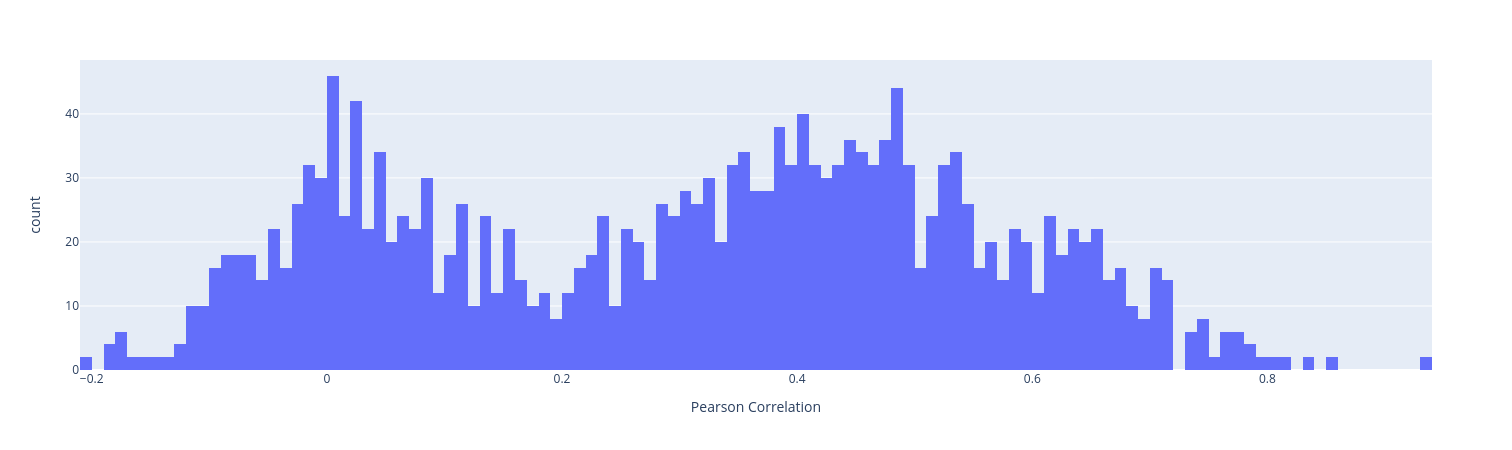
\includegraphics[scale=0.3]{images/correlation_hist.png}
    \caption{Histograma de correlación de los activos}
    \label{fig:hist_corr}
\end{figure}

\begin{figure}[htp]
    \centering
    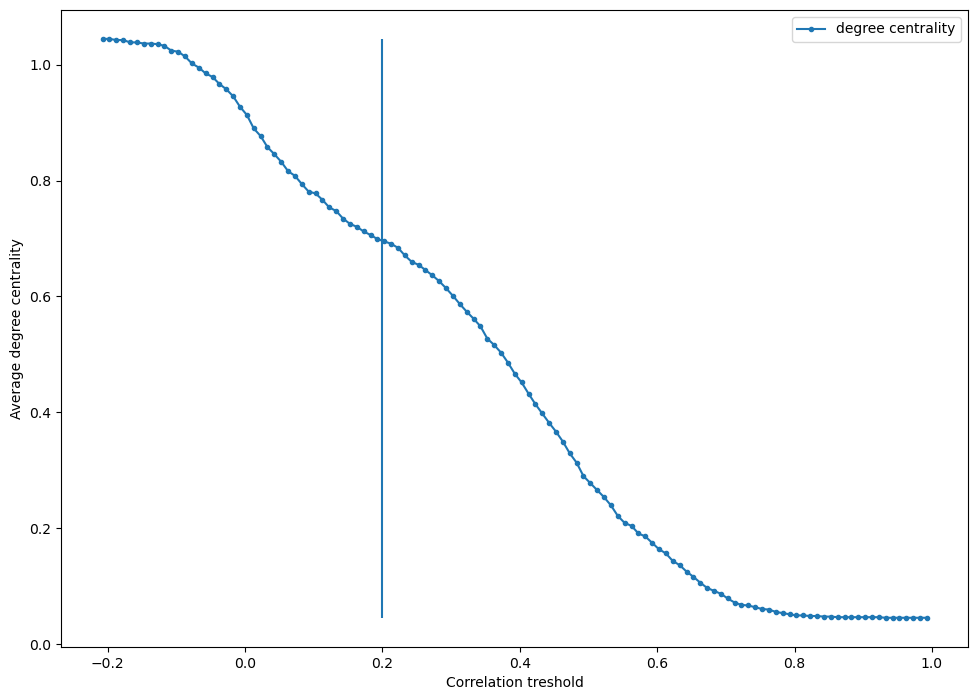
\includegraphics[scale=0.3]{images/degree_centrality.png}
    \caption{Ćentralidad}
    \label{fig:degree_centrality}
\end{figure}

\begin{figure}[htp]
    \centering
    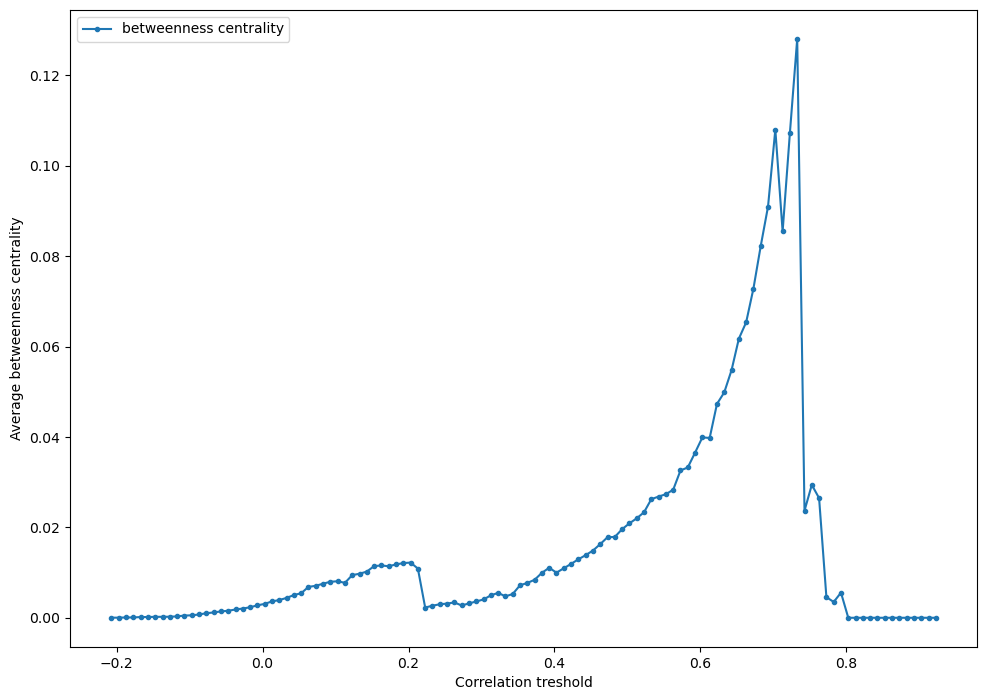
\includegraphics[scale=0.3]{images/betweeness_centrality.png}
    \caption{Ćentralidad de intermediación}
    \label{fig:btw_centrality}
\end{figure}


\begin{figure}[htp]
    \centering
    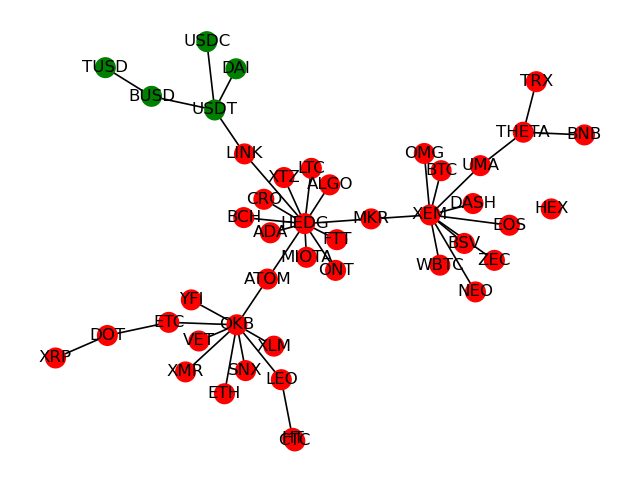
\includegraphics[scale=0.75]{images/mst.png}
    \caption{MST de los activos}
    \label{fig:mst}
\end{figure}

\begin{figure}[htp]
    \centering
    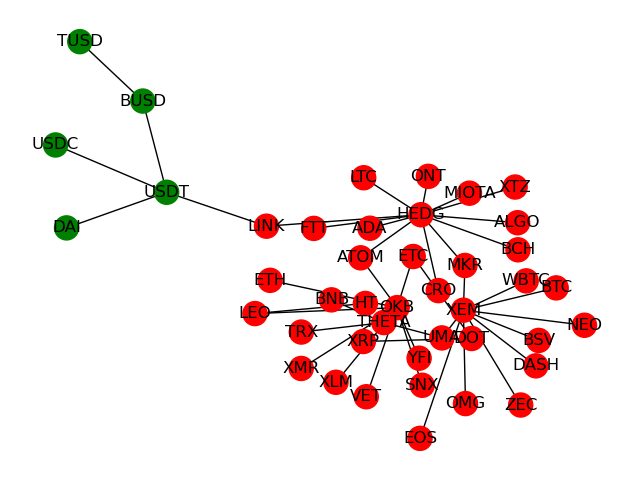
\includegraphics[scale=0.75]{images/community_louvain.png}
    \caption{Resultado del algoritmo Louvain}
    \label{fig:community_louvain}
\end{figure}

\begin{figure}[htp]
    \centering
    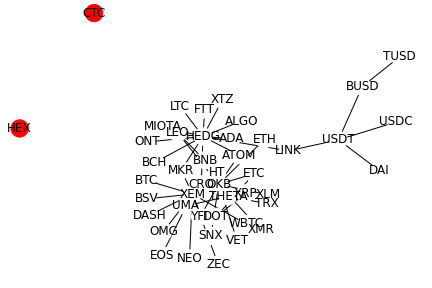
\includegraphics[scale=0.75]{images/community_gn.png}
    \caption{Resultado del algoritmo Girvan-Neuman}
    \label{fig:community_gn}
\end{figure}


\end{document}
